\chapter{Transmission d'un fichier binaire}
\minitoc
On insère un fichier txt sur la chaîne de transmission dans des conditions favorables, c'est à dire sans distorsion d'information.

\section{Résultats de la transmission sans distorsion}
En observant les fichiers file.txt (de  départ) et print.txt (d’arrivée), on constate :


\begin{itemize}
\item Les données obtenues en arrivée sont totalement déformées du fichier de base malgré qu'il s'agit d'une transmission sans bruit, les fichiers devant donc être identiques;
\item Le fichier de départ transmis par l'émetteur comprend des « 0 » et des « 1 » (codage RZ) tandis que le fichier d'arrivée comprend des valeurs flottantes de -1.0 et 1.0 (codage NRZ en flottant);
\item Il y a un retard (délai) de 16 bits;

\end{itemize}

\section{Correction de la transmission sans distorsion}
\paragraph{}
Afin d'obtenir des fichiers similaires pour poursuivre notre étude en sachant que tous les paramètre y sont convenablement fixés, nous procédons à une correction des erreurs du fichier d'arrivée.
\begin{itemize}
\item  Dans un premier temps, nous avons décidé d'insérer un bloc après le démodulateur qui convertirait les valeurs flottantes obtenues en entiers. Malgré cela, nous avions un fichier de départ en RZ et un en arrivée en NRZ, on en déduit que cette erreur provient du démodulateur. Car, il est chargé de retranscrire le fichier envoyé avec des niveaux de tensions données. Pour corriger cela, nous changeons donc son seuil de codage;
\item Toutefois, il subsiste un retard (délai) de 16 bits, retard dû aux deux filtres sur chaque ligne disposés en série, chacun d'eux insérant un retard de 8 bits à raison d'un bit pour 8 échantillons;
1 bit va être codé avec 8 échantillons ceci en sachant que nous avons un retard de 128 échantillons pour chacune des voies I et Q. Notons que la taille des filtres est représentatives de chaque retard, deux filtres de taille 64 sur chaque ligne, soient 128 échantillons de retard pour chaque voie, 16 bits.


\clearpage

\begin{figure}[bth]%[!ht]
\begin{center}
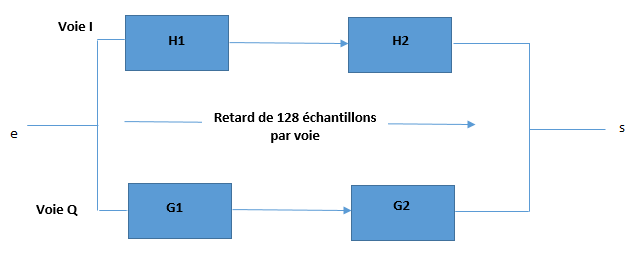
\includegraphics[scale=0.75]{filtres}%[height=70mm,width=70mm]
\caption{\textbf{Illustration du retard des filtres}}%
%\url {http://www.google.fr/}
\label{filtres}%
\end {center}
\end{figure}


Le calcul du TEB est bien évidemment déterminé en prenant en compte ce retard, c'est ce qui nous a permis d'en arriver à cette déduction et à retrouver les bits correspondants à ceux du fichier de départ.
\end{itemize}

